
\chapter{Multiblock Orthogonal Projections to Latent Structures}

\begin{quote}
{\it
  I see NIPALS as an open ended array of models with unlimited complexity
  in the combined use of several devices.}
\\\\
 -- Herman Wold
\end{quote}

\section{Introduction}

\begin{doublespace}
The method of nonlinear iterative partial least squares (NIPALS) has firmly
entrenched itself in the field of chemometrics. Implementations of principal
component analysis (PCA) and projections to latent structures (PLS) that
utilize NIPALS-type algorithms benefit from its numerical stability, as well
as its flexibility and simplicity
\cite{andersson:jchemo2009,hoskuldsson:jchemo1988,wold:cils2001}.
Only a few subroutines from level 2 of the basic linear algebra subprograms
(BLAS) specification are required to construct a complete NIPALS-type
algorithm \cite{golub2012}, making it an attractive means of constructing
PCA and PLS models of high-dimensional spectroscopic datasets.
\\\\
One particularly recent addition to the NIPALS family of algorithms, called
orthogonal projections to latent structures (OPLS), integrates an orthogonal
signal correction (OSC) filter into NIPALS PLS
\cite{trygg:jchemo2002,boulet:cils2012}. By extracting variation from its
computed PLS components that is uncorrelated (orthogonal) to the responses,
OPLS produces a more interpretable regression model compared to PLS. In fact,
when trained on the same data and responses, and OPLS model and a PLS model
with the same total number of components will show no difference in predictive
ability \cite{verron:jchemo2004}. Despite its relative novelty to the field,
the enhanced interpretability of OPLS over PLS has made it a popular method
in exploratory studies of spectroscopic datasets of complex chemical mixtures.
\\\\
Extensions of NIPALS PCA and PLS to incorporate blocking information that
partitions the set of measured variables into multiple `blocks' of data have
recently gained attention in the field, as more experimental designs involve
the collection of data from multiple analytical platforms per sample. In such
experiments, referred to as `class II' multiblock schemes by Smilde et al.
\cite{smilde:jchemo2003}, correlated consensus directions are sought from the
blocks that maximally capture block variation and (optionally) maximally
predict a set of responses. Of the available extensions of NIPALS to
multiblock modeling, a class of methods exists that bears attractive
computational qualities, namely computability from single-block bilinear
factorizations. When both super weights and block loadings are normalized in
consensus PCA (i.e. CPCA-W), the obtained super scores are equivalent to those
obtained from PCA of the concatenated matrix of blocks
\cite{westerhuis:jchemo1998}. Likewise, scores obtained from PLS of the
concatenated matrix are equivalent to super scores from multiblock PLS
(MB-PLS) when super scores are used in the deflation step
\cite{westerhuis:jchemo1997,westerhuis:jchemo1998}. As a result, these
multiblock bilinear factorizations inherit many of the useful properties
of their single-block equivalents.
\\\\
A second class of multiblock methods exists in which every block is predicted
in a regression model by every other block. In the first of such methods,
known as nPLS, the MAXDIFF criterion \cite{tenberge:psych1988} is optimized
one component at a time (i.e. sequentially) to yield a set of predictive
weight vectors for each block \cite{lofstedt:jchemo2011}. The recently
described OnPLS algorithm also falls within this class. OnPLS extends O2PLS
to three or more matrices and may be considered a prefixing of nPLS with an
OSC filtering step. OnPLS deflates non-globally predictive variation that
may or may not be orthogonal to all blocks from each matrix, and then computes
an nPLS model from the filtered result \cite{lofstedt:jchemo2011}. While fully
symmetric OnPLS is a powerful and general addition to the existing set of
multiblock modeling frameworks, it is arguably an over-complication when
the regression of a single response matrix on multiple data blocks
(i.e. MB-PLS) is sought. For such situations, a novel algorithm termed
MB-OPLS for multiblock orthogonal projections to latent structures is
introduced that embeds an OSC filter within NIPALS MB-PLS, thus solving an
inherently different problem from OnPLS. It will be shown that MB-OPLS, in
analogy to CPCA-W and MB-PLS, is computable from a single-block OPLS model
of the matrix of concatenated data blocks. Thus, MB-OPLS forms a bridge
between this special class of consensus component methods and the highly
general symmetric regression framework of OnPLS.
\end{doublespace}

\section{Theory}

\begin{doublespace}
MB-OPLS belongs to a set of multiblock methods that exhibit a computability
from their single-block equivalents. A short discussion of these methods
follows, in which the optimization criterion of each method is shown to
belong to the MAXBET family of objective functions. This is contrasted to
nPLS and OnPLS, which have been shown to optimize a MAXDIFF objective.
Finally, the equivalence of MB-OPLS and OPLS is demonstrated, and final
mentions are made to differences between MB-OPLS and OnPLS.
\\\\
In all following discussions, it will be understood that there exist $n$
data matrices $\mathbf{X}_1$ to $\mathbf{X}_n$, each having $N$ rows
(observations) and $K_i$ columns (variables). The matrix
$\mathbf{X} = [\mathbf{X}_1\mid\cdots\mid\mathbf{X}_n]$ of all concatenated
blocks will be used in cases of single-block modeling. Finally, a response
matrix $\mathbf{Y}$ having $N$ rows and $M$ columns will be assumed to exist
for the purposes of regression.
\end{doublespace}

\subsection{nPLS and OnPLS}

\begin{doublespace}
In their initial description of the OnPLS modeling framework
\cite{lofstedt:jchemo2011}, L\"{o}fstedt and Trygg introduced nPLS as a
generalization of PLS regression to cases where $n>2$, and a model is
sought in which each matrix $\mathbf{X}_i$ is predicted by all other
matrices $\mathbf{X}_{j \ne i}$. The nPLS solution involves indentifying
a set of weight vectors $\mathbf{w}_i$ that simultaneously maximmize the
covariances between each pair of resulting scores
$\mathbf{t}_i = \mathbf{X}_i \mathbf{w}_i$ via the following objective
function:
\begin{equation}
\sum_{\substack{i,j=1\\ i \ne j}}^n
 {\mathbf{t}_i}^T \mathbf{t}_j =
\sum_{\substack{i,j=1\\ i \ne j}}^n
 {\mathbf{w}_i}^T {\mathbf{X}_i}^T \mathbf{X}_j \mathbf{w}_j
\end{equation}
subject to the constraints $\|\mathbf{w}_i\|=1$. This objective was recognized
to be a member of the MAXDIFF family of functions, whose solution is obtainable
using a general algorithm from Hanafi and Kiers \cite{hanafi:csda2006}. After
the identification of a set of weight vectors, the scores
\begin{equation*}
\mathbf{t}_i = \mathbf{X}_i \mathbf{w}_i
\end{equation*}
and loadings
\begin{equation*}
\mathbf{p}_i = \frac{{\mathbf{X}_i}^T \mathbf{t}_i}
                    {{\mathbf{t}_i}^T \mathbf{t}_i}
\end{equation*}
may be computed for each matrix, which is then deflated prior to the
computation of subsequent component weights:
\begin{equation}
\mathbf{X}_i \gets \mathbf{X}_i - \mathbf{t}_i {\mathbf{p}_i}^T =
 \left( \mathbf{I} - \frac{\mathbf{t}_i {\mathbf{t}_i}^T}
                          {{\mathbf{t}_i}^T \mathbf{t}_i}
 \right) \mathbf{X}_i
\end{equation}

This deflation scheme follows the precedent set by two-block PLS regression.
Because their described approach used a distinct deflation scheme from
single-component (sequential) MAXDIFF, it was given the name `nPLS' by
the authors to distinguish it from MAXDIFF
\cite{lofstedt:jchemo2011,lofstedt2012}.
\\\\
OnPLS extends nPLS by decomposing each matrix into a globally predictive
part and a non-globally predictive (orthogonal) part using an orthogonal
projection. By removing orthogonal variation from each block prior to
constructing an nPLS model, OnPLS optimizes the following MAXDIFF-type
objective function:
\begin{equation}
\sum_{\substack{i,j=1\\ i \ne j}}^n
 {\mathbf{t}_i}^T \mathbf{t}_j =
\sum_{\substack{i,j=1\\ i \ne j}}^n
 {\mathbf{w}_i}^T {\mathbf{X}_i}^T \mathbf{Z}_i
  \mathbf{Z}_j \mathbf{X}_j \mathbf{w}_j
\end{equation}
where $\mathbf{Z}_i$ represents the orthogonal projector identified by
OnPLS for matrix $i$:
\begin{equation*}
\mathbf{Z}_i = \mathbf{I} - \mathbf{T_o}_i \left(
  {\mathbf{T_o}_i}^T \mathbf{T_o}_i
 \right)^{-1} {\mathbf{T_o}_i}^T
\end{equation*}
where
$\mathbf{T_o}_i = [\mathbf{t_o}_{i,1}\mid\cdots\mid\mathbf{t_o}_{i,A_o}]$,
the concatenation of all orthogonal score vectors for the block, and
$\mathbf{t_o}_{i,a} = \mathbf{X}_i \mathbf{w_o}_{i,a}$. In OnPLS, each
orthogonal weight $\mathbf{w_o}_{i,a}$ is chosen such that its score
$\mathbf{t_o}_{i,a}$ contains maximal covariance with the variation in
$\mathbf{X}_{j \ne i}$ that is not jointly predictive of $\mathbf{X}_i$.
The OnPLS framework provides a powerful set of methods for unsupervised
data mining and path modeling \cite{lofstedt:jchemo2011,lofstedt:jchemo2012,
  lofstedt:cils2012,lofstedt:aca2013}.
\end{doublespace}

\subsection{CPCA-W and MB-PLS}

\begin{doublespace}
The consensus PCA method, introduced by Wold et al. as CPCA and modified by
Westerhuis et al. into CPCA-W, identifies a set of weights $\mathbf{p}_i$
that maximally capture the within-block variances and between-block
covariances of a set of $n$ matrices \cite{westerhuis:jchemo1998}. It was
further proven by Westerhuis, Kourti and MacGregor that the results of CPCA-W
computed on matrices $\mathbf{X}_1$ to $\mathbf{X}_n$ are identical to those
from PCA of the concatenated matrix $[\mathbf{X}_1\mid\cdots\mid\mathbf{X}_n]$.
It immediately follows from this equivalence that the CPCA-W algorithm
optimizes the following objective function:
\begin{equation}
\mathbf{t}^T \mathbf{t} =
\mathbf{p}^T \mathbf{X}^T \mathbf{X} \mathbf{p} =
\sum_{i,j=1}^n {\mathbf{t}_i}^T \mathbf{t}_j =
\sum_{i,j=1}^n {\mathbf{p}_i}^T {\mathbf{X}_i}^T \mathbf{X}_j \mathbf{p}_j
\end{equation}
subject to the constraint $\|\mathbf{p}\|=1$, where
$\mathbf{p}^T=[{\mathbf{p}_1}^T\mid\cdots\mid{\mathbf{p}_n}^T]$. Maximizing
the above function yields a set of super scores $\mathbf{t}$ that relate the
$N$ observations in $\mathbf{X}$ to each other based on the extracted
consensus in $\mathbf{p}$, as well as block scores $\mathbf{t}_i$ and loadings
$\mathbf{p}_i$ that describe each block. This objective function is of the
MAXBET variety, in contrast to the MAXDIFF objective of nPLS and OnPLS. As
a result, the CPCA-W NIPALS algorithm may be considered a special case of
the general algorithm from Hanafi and Kiers \cite{hanafi:csda2006}.
\\\\
The multiblock PLS (MB-PLS) method, when deflation is performed using super
scores \cite{westerhuis:jchemo1997}, shares an equivalence with single-block
PLS as proven by Westerhuis et al. \cite{westerhuis:jchemo1998}. Therefore,
the MB-PLS objective takes on a similar form as in CPCA-W, with the addition
of a weighting matrix:
\begin{equation}
\mathbf{t}^T \mathbf{Y} \mathbf{Y}^T \mathbf{t} =
\mathbf{w}^T \mathbf{X}^T \mathbf{Y} \mathbf{Y}^T \mathbf{X} \mathbf{w} =
\sum_{i,j=1}^n
 {\mathbf{t}_i}^T \mathbf{Y} \mathbf{Y}^T \mathbf{t}_j =
\sum_{i,j=1}^n
 {\mathbf{w}_i}^T {\mathbf{X}_i}^T
  \mathbf{Y} \mathbf{Y}^T
 \mathbf{X}_j \mathbf{w}_j
\end{equation}
where once again $\|\mathbf{w}\|$ is constrained to unity. In analogy to
H\"{o}skuldsson's interpretation of PLS as a regression on orthogonal
components, where $\mathbf{Y}\mathbf{Y}^T$ is used to weight the covariance
matrix, the above function corresponds to a MAXBET objective with an inner
weighting of $\mathbf{Y}\mathbf{Y}^T$ \cite{hoskuldsson:jchemo1988}.
Alternatively, equation 9.5 could be interpreted as a MAXBET computed on the
$n$ cross-covariance matrices $\mathbf{Y}^T \mathbf{X}_1$ to
$\mathbf{Y}^T \mathbf{X}_n$.
\end{doublespace}

\subsection{MB-OPLS}

\begin{doublespace}
Extension of prior multiblock NIPALS algorithms to incorporate an OSC filter
rests on the observation that, in both the cases of CPCA-W and MB-PLS,
deflation of each computed component is accomplished using super scores.
For any super score deflation method, a loading vector is computed for each
block:
\begin{equation*}
\mathbf{p}_i = \frac{{\mathbf{X}_i}^T \mathbf{t}}
                    {\mathbf{t}^T \mathbf{t}}
\end{equation*}
and the super scores $\mathbf{t}$ and block loadings are then used to deflate
their respective block:
\begin{equation}
\mathbf{X}_i \gets \mathbf{X}_i - \mathbf{t} {\mathbf{p}_i}^T =
 \left( \mathbf{I} - \frac{\mathbf{t} \mathbf{t}^T}
                          {\mathbf{t}^T \mathbf{t}}
 \right) \mathbf{X}_i
\end{equation}

Equation 9.6 differs from equation 9.2 used in nPLS and OnPLS, which uses
block-specific scores and loadings during deflation. This method of super
score deflation ensures that the super scores become an orthogonal basis,
while allowing scores and loadings to become slightly correlated at the
block level, and is a necessary condition for the equivalences between
CPCA-W and MB-OPLS and their single-block counterparts
\cite{westerhuis:jchemo1998}. This condition shall be employed in MB-OPLS
by deflating each matrix by a set of orthogonal super scores $\mathbf{T_o}$,
which shall be shown to be equal to the orthogonal scores obtained from
single-block OPLS. By constructing an MB-PLS model on the set of matrices
after deflation by $\mathbf{T_o}$, we effectively arrive at another MAXBET
objective:
\begin{equation}
\mathbf{t}^T \mathbf{Y} \mathbf{Y}^T \mathbf{t} =
 \mathbf{w}^T \mathbf{X}^T \mathbf{Z} \mathbf{Y}
 \mathbf{Y}^T \mathbf{Z} \mathbf{X} \mathbf{w} =
\sum_{i,j=1}^n
 {\mathbf{t}_i}^T \mathbf{Y} \mathbf{Y}^T \mathbf{t}_j =
\sum_{i,j=1}^n
 {\mathbf{w}_i}^T {\mathbf{X}_i}^T \mathbf{Z}
  \mathbf{Y} \mathbf{Y}^T
 \mathbf{Z} \mathbf{X}_j \mathbf{w}_j
\end{equation}
where $\mathbf{w}$ is constrained to unit $\ell_2$-norm and $\mathbf{Z}$ is
the orthogonal projector for the super scores $\mathbf{T_o}$.
\end{doublespace}

\subsubsection{The MB-OPLS Model}

\begin{doublespace}
MB-OPLS constructs an OPLS model for each matrix $\mathbf{X}_i$, where the
predictive and orthogonal loadings for each matrix are interrelated by a
set of predictive and orthogonal super scores, respectively:
\begin{equation}
\mathbf{X}_i =
 \underbrace{\mathbf{T} {\mathbf{P}_i}^T}_{\mathbf{X_p}_i} +
 \underbrace{\mathbf{T_o} {\mathbf{P_o}_i}^T}_{\mathbf{X_o}_i} +
 \mathbf{E}_i
\end{equation}

Concatenation of all block-level matrices together in equation 9.8 results
in a top-level consensus model, which is in fact equivalent to an OPLS model
trained on the partitioned data matrix $\mathbf{X}$:
\begin{equation}
\mathbf{X} = [\mathbf{X}_1\mid\cdots\mid\mathbf{X}_n] =
 \underbrace{\mathbf{T} [{\mathbf{P}_1}^T\mid\cdots\mid{\mathbf{P}_n}^T]}
  _{\mathbf{X_p}} +
 \underbrace{\mathbf{T_o} [{\mathbf{P_o}_1}^T\mid\cdots\mid{\mathbf{P_o}_n}^T]}
  _{\mathbf{X_o}} +
 \underbrace{[\mathbf{E}_1\mid\cdots\mid\mathbf{E}_n]}_{\mathbf{E}}
\end{equation}

Like PLS, OPLS and MB-PLS, an MB-OPLS model contains a second equation that
relates the predictive super scores and responses:
\begin{equation}
\mathbf{Y} = \mathbf{T} \mathbf{C}^T + \mathbf{F}
\end{equation}
\end{doublespace}

\subsubsection{The MB-OPLS Algorithm}

\begin{doublespace}
The MB-OPLS algorithm was introduced in
\hyperlink{subsection.3.5.6}{Chapter 3}, but will be decomposed in more
detail as sub-algorithms here in order to relate it with the OPLS NIPALS
algorithm. MB-OPLS admits a matrix of responses $\mathbf{Y}$, but also
supports vector-$\mathbf{y}$ modeling as a special case. Direct and normed
assignment will be indicated by ``$\gets$'' and ``$\propto$'', respectively.
\end{doublespace}

\begin{algorithm}[H]
\caption{Core Algorithm for MB-OPLS}
\label{algorithm.9.1}
\begin{algorithmic}[1]
\REQUIRE $\{\mathbf{X}_i \in \mathbb{R}^{N \times K_i}\}_{i=1}^n$,%
         $\:\mathbf{Y} \in \mathbb{R}^{N \times M}$
\STATE $\mathbf{V}_i \gets \text{SUBSPACE}(\mathbf{X}_i, \mathbf{Y})
        \quad \forall i \in \{1, \dots, n\}$
\STATE $\{\mathbf{w}_i\}_{i=1}^n,
        \{\mathbf{t}_i\}_{i=1}^n,
        \{\mathbf{p}_i\}_{i=1}^n,
        \mathbf{t}, \mathbf{c}, \mathbf{u} \gets
        \text{PREDCMP}(\{\mathbf{X}_i\}_{i=1}^n, \mathbf{Y})$
\STATE{
  To compute an orthogonal component, continue to step (4). \\
  Otherwise, proceed to step (7).
}
\STATE $\{\mathbf{w_o}_i\}_{i=1}^n,
        \{\mathbf{t_o}_i\}_{i=1}^n,
        \{\mathbf{p_o}_i\}_{i=1}^n,
        \mathbf{t_o} \gets
        \text{ORTHCMP}(\{\mathbf{X}_i\}_{i=1}^n,
                       \{\mathbf{V}_i\}_{i=1}^n,
                       \{\mathbf{p}_i\}_{i=1}^n)$
\STATE $\mathbf{X}_i \gets \mathbf{X}_i - \mathbf{t_o} {\mathbf{p_o}_i}^T
        \quad \forall i \in \{1, \dots, n\}$
\STATE{Return to step (2).}
\STATE $\mathbf{X}_i \gets \mathbf{X}_i - \mathbf{t} \mathbf{p}_i^T
        \quad \forall i \in \{1, \dots, n\}$
\STATE{
  To compute another predictive component, return to step (2). \\
  Otherwise, end.
}
\end{algorithmic}
\end{algorithm}

\begin{doublespace}
The SUBSPACE method computes the $\mathbf{Y}$-predictive subspace
for each data matrix $\mathbf{X}_i$, and follows directly from
single-block OPLS:
\end{doublespace}

\begin{algorithm}[H]
\caption{Predictive Subspace Identification for MB-OPLS}
\label{algorithm.9.2}
\begin{algorithmic}[1]
\REQUIRE $\mathbf{X} \in \mathbb{R}^{N \times K}$,%
       $\:\mathbf{Y} \in \mathbb{R}^{N \times M}$
\FORALL{$m \in \{1, \dots, M\}$}
  \STATE $\mathbf{v}_m \gets \mathbf{X}^T \mathbf{y}_m
          \cdot \left( \mathbf{y}_m^T \mathbf{y}_m \right)^{-1}$
  \STATE $\mathbf{V} \gets [\mathbf{V} \mid \mathbf{v}_m]$
\ENDFOR
\end{algorithmic}
\end{algorithm}

\begin{doublespace}
Predictive MB-OPLS components identified by the PREDCMP method are, in fact,
MB-PLS components:
\end{doublespace}

\begin{algorithm}[H]
\caption{Predictive Component Computation for MB-OPLS}
\label{algorithm.9.3}
\begin{algorithmic}[1]
\REQUIRE $\{\mathbf{X}_i \in \mathbb{R}^{N \times K_i}\}_{i=1}^n$,%
         $\:\mathbf{Y} \in \mathbb{R}^{N \times M}$
\STATE{Initialize $\mathbf{u}$ to a column of $\mathbf{Y}$}
\REPEAT
  \STATE $\mathbf{w}_i \propto {\mathbf{X}_i}^T \mathbf{u}
          \quad \forall i \in \{1, \dots, n\}$
  \STATE $\mathbf{t}_i \gets \mathbf{X}_i \mathbf{w}_i
          \quad \forall i \in \{1, \dots, n\}$
  \STATE $\mathbf{R} \gets [\mathbf{t}_1 \mid\cdots\mid \mathbf{t}_n]$
  \STATE $\mathbf{w_T} \propto \mathbf{R}^T \mathbf{u}$
  \STATE $\mathbf{t} \gets \mathbf{R} \mathbf{w_T}$
  \STATE $\mathbf{c} \gets
          \left( \mathbf{Y}^T \mathbf{t} \right) \cdot
          \left( \mathbf{t}^T \mathbf{t} \right)^{-1}$
  \STATE $\mathbf{u} \gets
          \left( \mathbf{Y} \mathbf{c} \right) \cdot
          \left( \mathbf{c}^T \mathbf{c} \right)^{-1}$
\UNTIL{
  $\|\mathbf{u} - \mathbf{u}_{old}\|
   \cdot \|\mathbf{u}_{old}\|^{-1} < \varepsilon$
}
\STATE $\mathbf{p}_i \gets
        \left( {\mathbf{X}_i}^T \mathbf{t} \right) \cdot
        \left( \mathbf{t}^T \mathbf{t} \right)^{-1}
        \quad \forall i \in \{1, \dots, n\}$
\end{algorithmic}
\end{algorithm}

\begin{doublespace}
In the above method, the value of $\varepsilon$ is set to a very small
number, such as $10^{-9}$. Once a predictive component has been computed,
MB-OPLS uses the ORTHCMP method to extract a new orthogonal component:
\end{doublespace}

\begin{algorithm}[H]
\caption{Orthogonal Component Computation for MB-OPLS}
\label{algorithm.9.4}
\begin{algorithmic}[1]
\REQUIRE $\{\mathbf{X}_i \in \mathbb{R}^{N \times K_i}\}_{i=1}^n$,%
       $\:\{\mathbf{V}_i \in \mathbb{R}^{M \times K_i}\}_{i=1}^n$,%
       $\:\{\mathbf{p}_i \in \mathbb{R}^{K_i}\}_{i=1}^n$
\STATE $\mathbf{w_o}_i \gets \mathbf{p}_i
        \quad \forall i \in \{1, \dots, n\}$
\FORALL{$m \in \{1, \dots, M\}$}
  \STATE $\phi \gets
      \left( \sum_{i=1}^n {\mathbf{v}_{i,m}}^T \mathbf{w_o}_i \right) \cdot
      \left( \sum_{i=1}^n {\mathbf{v}_{i,m}}^T \mathbf{v}_{i,m} \right)^{-1}$
  \STATE $\mathbf{w_o}_i \gets \mathbf{w_o}_i - \phi \mathbf{v}_{i,m}
          \quad \forall i \in \{1, \dots, n\}$
\ENDFOR
\STATE $\alpha \gets \left(
         \sum_{i=1}^n {\mathbf{w_o}_i}^T \mathbf{w_o}_i
        \right)^{-1/2}$
\STATE $\mathbf{w_o}_i \gets \alpha \mathbf{w_o}_i
        \quad \forall i \in \{1, \dots, n\}$
\STATE $\mathbf{t_o}_i \gets \mathbf{X}_i \mathbf{w_o}_i
        \quad \forall i \in \{1, \dots, n\}$
\STATE $\mathbf{t_o} \gets \sum_{i=1}^n \mathbf{t_o}_i$
\STATE $\mathbf{p_o}_i \gets
        \left( {\mathbf{X}_i}^T \mathbf{t_o} \right) \cdot
        \left( \mathbf{t_o}^T \mathbf{t_o} \right)^{-1}
        \quad \forall i \in \{1, \dots, n\}$
\end{algorithmic}
\end{algorithm}

\begin{doublespace}
For each predictive component in the model, a set of orthogonal components is
extracted. After the computation of a new orthogonal component, the current
predictive component is updated to reflect the removal of orthogonal variation
from the matrices $\mathbf{X}_i$. The MB-OPLS algorithm closely follows the
matrix-$\mathbf{Y}$ OPLS algorithm presented by Trygg and Wold
\cite{trygg:jchemo2002}, but replaces the standard PLS computation
(steps 4--10 in OPLS) with an MB-PLS computation.
\end{doublespace}

\subsubsection{Equivalence to OPLS}

\begin{doublespace}
In both the vector-$\mathbf{y}$ and matrix-$\mathbf{Y}$ OPLS algorithms
proposed by Trygg and Wold \cite{trygg:jchemo2002}, a basis $\mathbf{V}$
for the response-correlated variation in $\mathbf{X}$ is constructed by
regressing the data onto each column of responses:
\begin{equation}
\mathbf{v}_m \gets \frac{\mathbf{X}^T \mathbf{y}_m}
                        {{\mathbf{y}_m}^T \mathbf{y}_m}
 \quad \forall m \in \{1, \dots, M\}
\end{equation}
where $\mathbf{y}_m$ and $\mathbf{v}_m$ denote the $m$-th columns of
$\mathbf{Y}$ and $\mathbf{V}$, respectively. When $\mathbf{X}$ is partitioned
into multiple blocks, the computed basis also bears the same partitioning,
i.e. $\mathbf{V}^T=[{\mathbf{V}_1}^T\mid\cdots\mid{\mathbf{V}_n}^T]$, where
each of the $n$ submatrices corresponds to the regression of its respective
block $\mathbf{X}_i$ onto the responses:
\begin{equation}
\mathbf{v}_{i,m} \gets \frac{{\mathbf{X}_i}^T \mathbf{y}_m}
                            {{\mathbf{y}_m}^T \mathbf{y}_m}
 \quad \forall m \in \{1, \dots, M\}
\end{equation}
where $\mathbf{v}_{i,m}$ is the $m$-th column of $\mathbf{V}_i$. Therefore,
the bases of response-correlated variation identified by OPLS and MB-OPLS
are equal. Given a single-block PLS loading vector $\mathbf{p}$, the OPLS
algorithm computes an orthogonal weight $\mathbf{w_o}$ by orthogonalizing
$\mathbf{p}$ to the columns of $\mathbf{V}$:
\begin{equation}
\mathbf{w_o} \gets \mathbf{w_o} - \left(
 \frac{{\mathbf{v}_m}^T \mathbf{w_o}}
      {{\mathbf{v}_m}^T \mathbf{v}_m}
 \right) \cdot \mathbf{v}_m
 \quad \forall m \in \{1, \dots, M\}
\end{equation}
after $\mathbf{w_o}$ has been initialized from $\mathbf{p}$. From the proof
of Westerhuis et al. \cite{westerhuis:jchemo1998}, it is known that the
single-block PLS loading $\mathbf{p}$ equals the concatenation of all block
loadings from MB-PLS, i.e. that
$\mathbf{p}^T=[{\mathbf{p}_1}^T\mid\cdots\mid{\mathbf{p}_n}^T]$. Expansion
of all vector terms in the above equation into their partitioned forms
results in the following new assignment rule:
\begin{equation}
\mathbf{w_o}_i \gets \mathbf{w_o}_i - \left(
 \frac{\sum_{i=1}^n {\mathbf{v}_{i,m}}^T \mathbf{w_o}_i}
      {\sum_{i=1}^n {\mathbf{v}_{i,m}}^T \mathbf{v}_{i,m}}
 \right) \cdot \mathbf{v}_{i,m}
 \quad \forall m \in \{1, \dots, M\}
\end{equation}

The scalar term in equation 9.14 should be recognized as $\phi$ in the
ORTHCMP method. By the same reasoning, steps 6 and 7 in ORTHCMP are
equivalent to scaling $\mathbf{w_o}$ to unit norm. Therefore, because
$\mathbf{w_o}$ is the column-wise concatenation of all weights
$\mathbf{w_o}_i$, it is then apparent that the orthogonal super scores
extracted by MB-OPLS are identical to those from OPLS of the concatenated
matrix $\mathbf{X}$:
\begin{equation}
\mathbf{t_o} = \mathbf{X} \mathbf{w_o} =
 [\mathbf{X}_1 \mid\cdots\mid \mathbf{X}_n]
 \begin{bmatrix}
  \mathbf{w_o}_1 \\
  \vdots \\
  \mathbf{w_o}_n
 \end{bmatrix}
 = \sum_{i=1}^n \mathbf{X}_i \mathbf{w_o}_i
 = \sum_{i=1}^n \mathbf{t_o}_i
\end{equation}

From this equivalence, and the fact that PREDCMP in MB-OPLS constitutes an
MB-PLS computation, we arrive at the equivalence between MB-OPLS and OPLS.
Thus, orthogonality between the responses and orthogonal super scores
$\mathbf{t_o}$ computed by MB-OPLS is also ensured. However, because the
computation of orthogonal weights involves all blocks, the resulting
orthogonal block scores $\mathbf{t_o}_i$ are not guaranteed to be orthogonal
to the responses.
\end{doublespace}

\subsubsection{Computation from an OPLS Model}

\begin{doublespace}
The equivalence between MB-OPLS super scores and OPLS scores may be leveraged
to generate an MB-OPLS model from an existing OPLS model of a partitioned
data matrix, saving computation time during cross-validated model training.
Algorithm 3.7 in \hyperlink{subsection.3.5.6}{Chapter 3} details the
extraction of MB-OPLS block scores and loadings from an OPLS model.
\\\\
The keen observer will recognize the similarity between Algorithm 3.7 and the
procedure outlined by Westerhuis et al. for extracting MB-PLS block components
from a PLS model \cite{westerhuis:jchemo1998}. By using this algorithm to
compute MB-OPLS models, the analyst avoid the unnecessary computation of
block components during cross-validated model training.
\end{doublespace}

\section{Datasets}

\begin{doublespace}
Two datasets will be described to illustrate how MB-OPLS effectively
integrates an OSC filter into an MB-PLS decomposition of a set of $n$
matrices. The first synthetic dataset contrasts the mixing of predictive
information in MB-PLS with its separation in MB-OPLS using a contrived
three-block regression example similar to that introduced by L\"{o}fstedt
and Trygg \cite{lofstedt:jchemo2011}. The second dataset, a joint set of
NMR and MS observations introduced in \hyperlink{section.4.3}{Chapter 4},
is used to demonstrate the enhanced interpretability of MB-OPLS models
over MB-PLS in a real example of discriminant analysis. All modeling and
validation were performed using routines available in the MVAPACK
chemometrics toolbox \cite{worley:acscb2014}.
\end{doublespace}

\begin{figure}[ht!]
\includegraphics[width=6.5in]{figs/mbopls/01-synthetic.png}
\caption
      [Synthetic Three-block Example Dataset.]{
  {\bf Synthetic Three-block Example Dataset.}
  \\
  Block loadings in the synthetic multiblock example dataset.
  ({\bf A}) True predictive loadings (solid) and sorthogonal loadings (dashed)
  used to construct the three-block dataset. First, second and third block
  loadings are colored in red, green and blue, respectively.
  ({\bf B}) First component (solid) and second component (dashed) loadings
  identified by MB-PLS modeling of the three data blocks.
  ({\bf C}) Predictive (solid) and orthogonal (dashed) block loadings
  identified by MB-OPLS, illustrating the separation of
  $\mathbf{y}$-uncorrelated variation accomplished by the integrated
  OSC filter.
}
\label{figure.9.1}
\end{figure}

\subsection{Synthetic Example}

\begin{doublespace}
In the first dataset, three matrices (all having 100 rows and 200 columns)
were constructed to hold one $\mathbf{y}$-predictive component
($\mathbf{t} {\mathbf{p}_i}^T$) and one $\mathbf{y}$-orthogonal component
($\mathbf{t_o} {\mathbf{p_o}_i}^T$). The score vectors were non-overlapping
(orthogonal) Gaussian density functions, and all block loading vectors were
mutually overlapping Gaussian density or square step functions. The true
synthetic block loadings are illustrated in \figref{9.1}{Figure 9.1A}.
A two-component MB-PLS-R model was trained on the synthetic three-block
example dataset, as well as a $1+1$ (one predictive, one orthogonal)
component MB-OPLS-R model. Block loadings extracted by MB-PLS-R and
MB-OPLS-R and shown in \figref{9.1}{Figures 9.1B} and
\figref{9.1}{9.1C}, respectively.
\end{doublespace}

\subsection{Joint \hnmr{} NMR and DI-ESI-MS Datasets}

\begin{doublespace}
The second dataset is a pair of processed and treated data matrices, collected
on 29 samples of metabolite extracts from human dopaminergic neuroblastoma
cells treated with various neurotoxic agents \cite{lei:acscb2014}. Details
about the collection, processing and treatment of this dataset may be found
in \hyperlink{section.4.3}{Chapter 4}, but will be resummarized here. The
first matrix, collected using \hnmr{} NMR spectroscopy, contains 16,138
columns and the second, collected using direct injection electrospray
ionization mass spectrometry (DI-ESI-MS), contains 2,095 columns. Prior
to all modeling, block weighting was applied after Pareto scaling to ensure
equal contribution of each block to the models \cite{smilde:jchemo2003}.
\\\\
In a previously published analysis of this dataset \cite{marshall:metab2015},
a two-component, two-class (vector-$\mathbf{y}$) MB-PLS-DA model was trained
on the dataset in order to discriminate between untreated and
neurotoxin-treated cell samples. To highlight the improved interpretability
of MB-OPLS over MB-PLS, a $1+1$ MB-OPLS-DA model was trained on the data
using an identical vector of class labels. Block components were extracted
from an OPLS-DA model of the concatenated matrix
$\mathbf{X}=[\mathbf{X}_{NMR}\mid\mathbf{X}_{MS}]$ using Algorithm 3.7 in
\hyperlink{subsection.3.5.6}{Chapter 3}. For both models, fifty rounds of
Monte Carlo seven-fold cross-validation \cite{shao:jasa1993,xu:cils2001}
were performed to compute per-component \qsq{} statistics
\cite{wold:cils2001}, in addition to the \rsq{} statistics available
from model training. CV-ANOVA significance testing was also applied
to further assess model reliability \cite{eriksson:jchemo2008}.
\end{doublespace}

\begin{figure}[ht!]
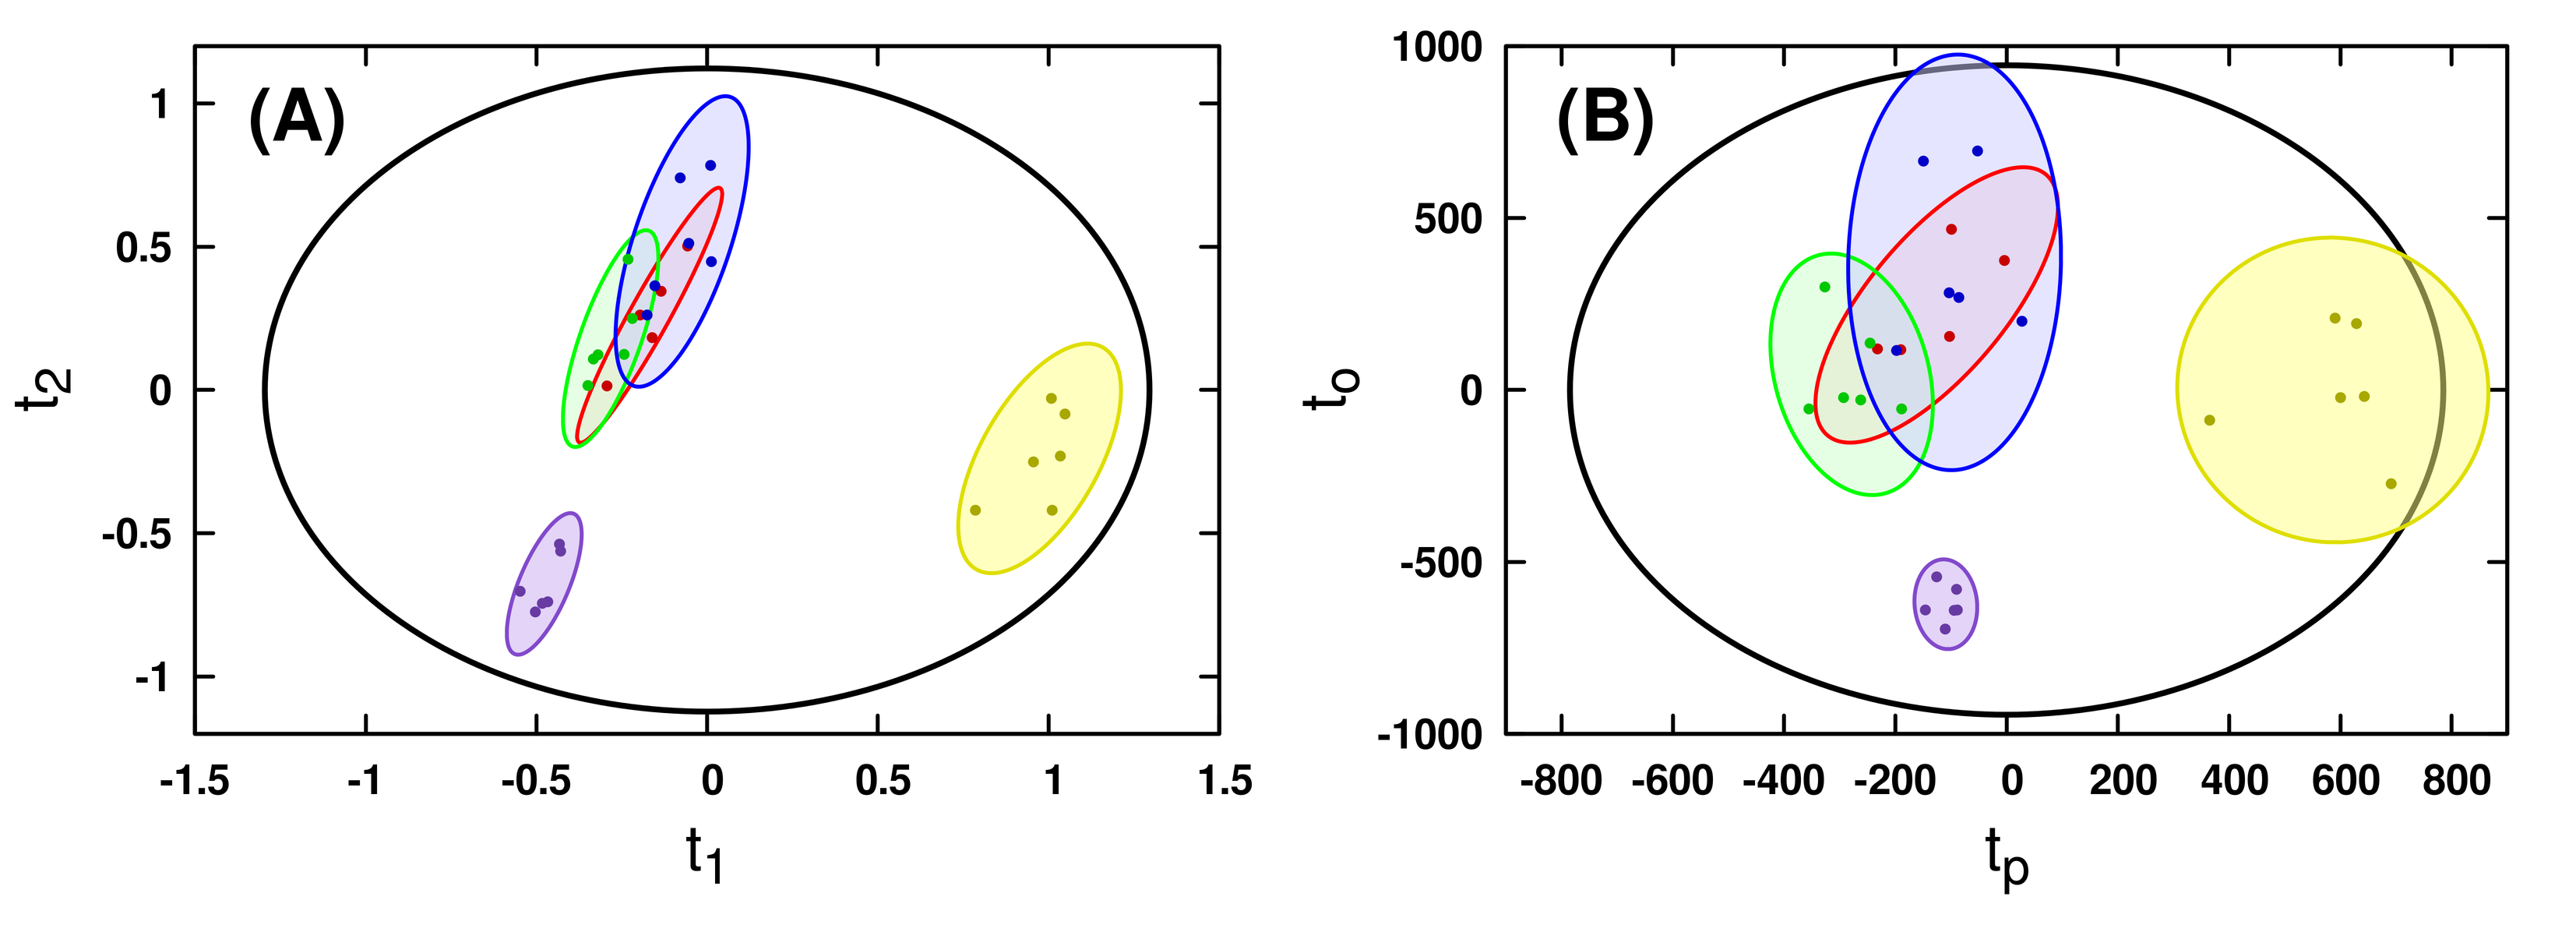
\includegraphics[width=6.5in]{figs/mbopls/02-scores.png}
\caption
      [Super Scores of Joint Spectroscopic Data.]{
  {\bf Super Scores of Joint Spectroscopic Data.}
  \\
  Super scores identified by ({\bf A}) MB-PLS and ({\bf B}) MB-OPLS modeling
  of the joint \hnmr{} NMR and DI-ESI-MS data matrices. Extraction of
  $\mathbf{y}$-orthogonal variation from the first PLS component is
  clear in the MB-OPLS scores. Ellipses represent the 95\% confidence
  regions for each sub-class of observations, assuming normal distributions.
  Colors indicate membership to the untreated (yellow), 6-hydroxydopamine
  (red), 1-methyl-4-phenylpyridinium (green) and paraquat (violet)
  sub-classes. Cross-validated super scores are shown in Figure 9.3.
}
\label{figure.9.2}
\end{figure}

\begin{figure}[ht!]
\includegraphics[width=6.5in]{figs/mbopls/03-cvscores.png}
\caption
      [Cross-validated Super Scores of Joint Spectroscopic Data.]{
  {\bf Cross-validated Super Scores of Joint Spectroscopic Data.}
  \\
  Cross-validation estimated super scores from ({\bf A}) MB-PLS and ({\bf B})
  MB-OPLS modeling of the joint \hnmr{} NMR and DI-ESI-MS data matrices.
  Points indicate mean values for each observation, and filled regions
  represent the union of all observations' confidence intervals from
  Monte Carlo iterations. Class colors are identical to those in
  Figure 9.2.
}
\label{figure.9.3}
\end{figure}

\section{Results and Discussion}

\begin{doublespace}
In both the contrived dataset and the real spectroscopic dataset, the
interpretative advantage offered by MB-OPLS over MB-PLS is strikingly
apparent. In the synthetic example, MB-OPLS capably identifies the true
predictive and orthogonal loadings in the presence of $\mathbf{y}$-orthogonal
variation that clouds the interpretation of MB-PLS loadings
(\figref{9.1}{Figure 9.1}). By design, this comparison between
MB-OPLS and MB-PLS is highly similar to the first example
presented by L\"{o}fstedt and Trygg to compare nPLS and OnPLS
for general data discovery \cite{lofstedt:jchemo2011}. However, as is
evidenced by the differences between equations 9.3 and 9.7 above, MB-OPLS
solves an inherently distinct problem from OnPLS: the identification of
consensus variation in multiple blocks of data that predicts a single set
of responses.
\\\\
The ability of MB-OPLS to separate predictive and orthogonal variation from
multiple data matrices is further exemplified in the discriminant analysis
of the real spectroscopic dataset. From the rotated discrimination axis in
the MB-PLS-DA scores (\figref{9.2}{Figure 9.2A}), it is clear that predictive
and orthogonal variation have become mixed in the corresponding block loadings
(\figref{4.11}{Figure 4.11}). Integration of an OSC filter into the multiblock
model in the form of MB-OPLS-DA achieved the expected rotation of super scores
to place more predictive variation into the first component
(\figref{9.2}{Figure 9.2B}). As a consequence of this rotation, spectral
information that separates paraquat treatment from other neurotoxin treatments
is also moved into the orthogonal component. For example, strong loadings from
citrate in the \hnmr{} NMR MB-PLS block loadings
(\figref{4.11}{Figure 4.11A}, 2.6 ppm) are substantially diminished
in the predictive block loadings from MB-OPLS
(\figref{4.12}{Figure 4.12A}), as separation between paraquat and
other treatments has been isolated along the orthogonal component in super
scores. Inspection of the orthogonal block loadings from MB-OPLS
(\figref{4.13}{Figure 4.13}) will reveal, as expected, that citrate
contributes more to separation between neurotoxin treatments than to
separation between treatments and controls.
\\\\
The partial correlation of both predictive and orthogonal block scores in
MB-OPLS is readily observed in the comparison of block scores from MB-PLS
and MB-OPLS (\figref{9.4}{Figures 9.4} and \figref{9.5}{9.5}). While the
super scores in \figref{9.2}{Figure 9.2B} are rotated to separate predictive
and orthogonal variation, block scores in \figref{9.4}{Figures 9.4B} and
\figref{9.5}{9.5B} have slightly rotated back into alignment with
the MB-PLS block scores. This partial correlation and re-mixing of
predictive and orthogonal variation in MB-OPLS block scores is a consequence
of the use of super score deflation in the presented algorithm. When all
matrices contain similar patterns of orthogonal variation, their MB-OPLS
block scores will reflect this by retaining the OSC-induced rotation captured
at the consensus level by the super scores.
\\\\
Because the MB-OPLS-DA model of the real spectral data matrices was trained
using the single-block OPLS routine already present in MVAPACK, all standard
cross-validation metrics were available in the model without further
computational expenditure. Monte Carlo cross-validation of the MB-PLS model
produced cumulative \rsqy{} and \qsq{} statistics of 0.988 and
0.901$\pm$0.015, respectively, and validation of the MB-OPLS model resulted
in statistics of 0.903 and 0.706$\pm$0.028, respectively. In addition, MB-OPLS
modeling yielded \rsqxp{} and \rsqxo{} statistics of 0.378 and 0.245 for the
first block, and 0.236 and 0.083 for the second block. Monte Carlo
cross-validated super scores from MB-PLS and MB-OPLS are depicted in
\figref{9.2}{Figure 9.2}. Compared to MB-PLS scores in
\figref{9.2}{Figure 9.2A}, MB-OPLS scores
(\figref{9.2}{Figure 9.2B}) exhibit an increased uncertainty due to the
coupled nature of predictive and orthogonal components in OPLS models.
Further validation of the MB-OPLS-DA model via CV-ANOVA produced
a $p$ value equal to $2.88 \times 10^{-6}$, indicating a sufficiently
reliable model.
\\\\
It is worthy of final mention that the objective solved by MB-OPLS is but a
single member of a superfamily of methods introduced in detail by Hanafi
and Kiers \cite{hanafi:csda2006}. In the first family, nPLS and OPLS maximally
capture the between-matrix covariances before and after orthogonal signal
correction, respectively, and thus serve to regress a set of matrices
against each other. Methods in the second family capture \emph{both}
within-matrix variances and between-matrix covariances of a set of matrices
(CPCA-W), a set of response-weighted matrices (MB-PLS), and a set of
response-weighted OSC-filtered matrices (MB-OPLS). By casting these methods
in the light of MAXDIFF and MAXBET, we obtain an informative picture of their
characteristics, commonalities, and differences. For example, nPLS and OnPLS
force an equal contribution of each matrix to the solution through the
constraint $\|\mathbf{w}_i\|=1$, while CPCA-W, MB-PLS and MB-OPLS allow
contributions to float based on the `importance' of each matrix to the
modeling problem at hand. This super weight approach necessitates a block
scaling procedure to avoid highly weighting any given matrix due to size
alone \cite{smilde:jchemo2003,westerhuis:jchemo1998}.
\end{doublespace}

\begin{figure}[ht!]
\includegraphics[width=6.5in]{figs/mbopls/04-blkscores-1.png}
\caption
      [First-block Scores of Joint Spectroscopic Data.]{
  {\bf First-block Scores of Joint Spectroscopic Data.}
  \\
  Block scores from ({\bf A}) MB-PLS and ({\bf B}) MB-OPLS modeling of the
  \hnmr{} NMR data matrix. Ellipses and class colors are identical to those
  in Figure 9.2.
}
\label{figure.9.4}
\end{figure}

\begin{figure}[ht!]
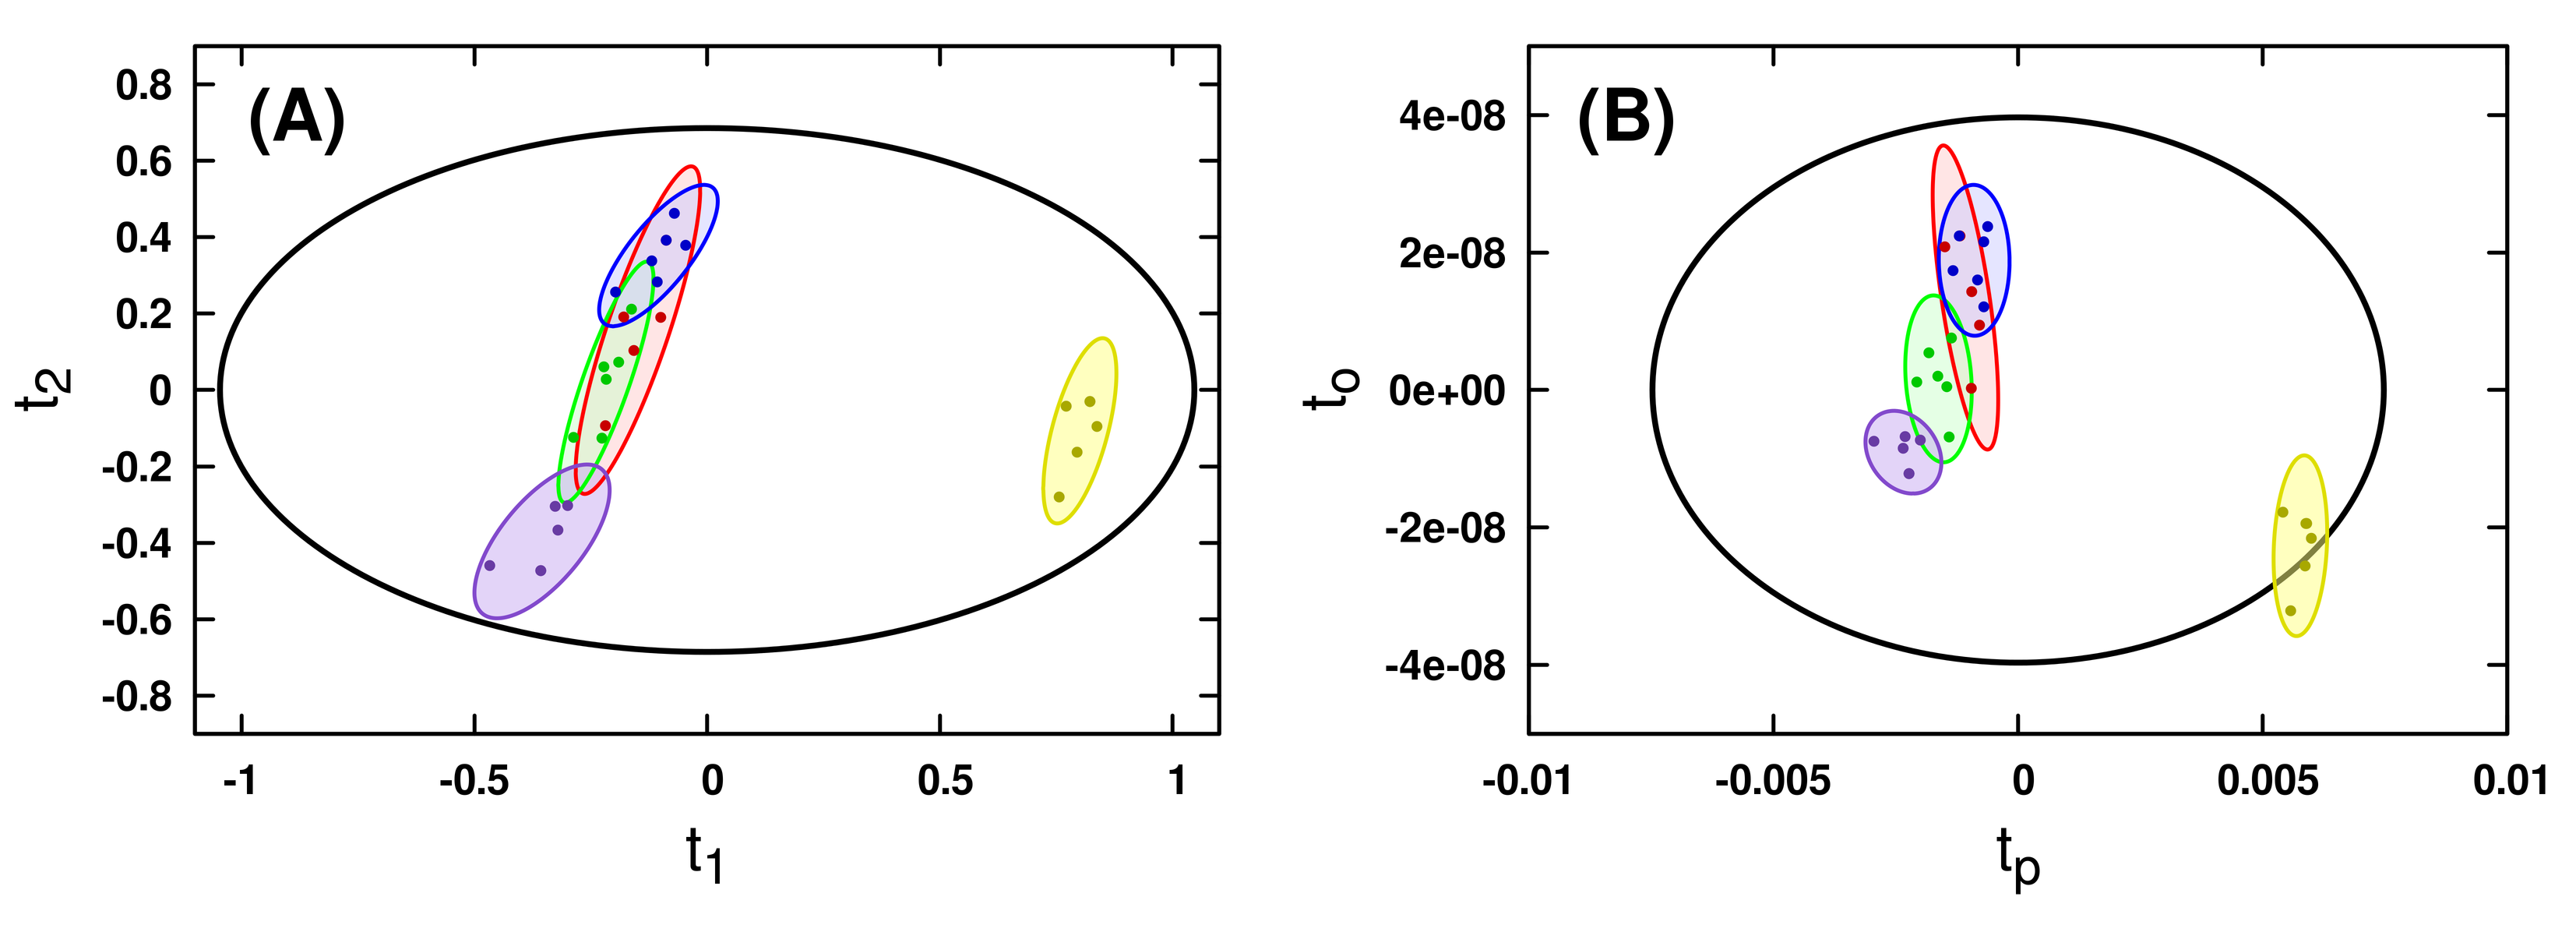
\includegraphics[width=6.5in]{figs/mbopls/05-blkscores-2.png}
\caption
      [Second-block Scores of Joint Spectroscopic Data.]{
  {\bf Second-block Scores of Joint Spectroscopic Data.}
  \\
  Block scores from ({\bf A}) MB-PLS and ({\bf B}) MB-OPLS modeling of the
  DI-ESI-MS data matrix. Ellipses and class colors are identical to those
  in Figure 9.2.
}
\label{figure.9.5}
\end{figure}

\section{Conclusions}

\begin{doublespace}
The MB-OPLS method described in this chapter is a versatile extension of
MB-PLS to include an OSC filter, and belongs to a family of MAXBET optimizers
that share an equivalence with their single-block factorizations. By removing
consensus response-uncorrelated variation from a set of $n$ data matrices,
MB-OPLS expands the scope and benefits of OPLS to cases where blocking
information is available. The ability of MB-OPLS to separate predictive and
orthogonal variation from multiple blocks of data has been demonstrated on
both synthetic and real spectral data, both in cases of vector-$\mathbf{y}$
regression and discriminant analysis. The described algorithm admits either
a vector or a matrix as responses, and is implemented in the latest version
of the open-source MVAPACK chemometrics toolbox \cite{worley:acscb2014}.
\end{doublespace}

\bibliographystyle{abbrv}
\bibliography{bworley}

